% !TEX root = ../Article.tex
\section{Setup}
In order to do research on how smart cards can have an impact on mobile data security and to perform an evaluation on how effective they are we need to have a proper test environment. We define "proper test environment" as an environment as close to reality as possible.
\subsection{Equipment}
\label{sec:equipment}

\paragraph{Test device}\mbox{}\\
The device we will be using for deploying the applications and performing tests on is considered to be a mid-range device. The device is a Sony Xperia M2 Aqua smartphone running Android 5.1.1 with the following relevant specifications:
\begin{itemize}
    \item Chipset: Qualcomm MSM8926-2 Snapdragon 400
    \item CPU: Quad-core 1.2 GHz Cortex-A7
    \item RAM: 1 GB
\end{itemize}
More information on the specifications of the phone can be found on  \newline
GSMArena.com \cite{sonym2}.

\paragraph{Java smart card}\mbox{}\\
We will be using two types of smart cards. The first type is a micro SD memory card (IDCore 8030 MicroSD card) as shown in figure \ref{fig:msdcard} produced by Gemalto. The reasoning for using this card for testing is that Gemalto delivers ready-to-use cards along with a framework for communicating with them. The cards we will be using have nothing pre-installed on them and we can freely deploy custom applications to the card. In order to use the provided framework we need a key provided by Gemalto which has a validity period of 120 days.

The second type of card we will be using is a plain hybrid smart card (ref. figure \ref{fig:nfccard}) with no pre-installed software which is also provided by Gemalto along with a standard card reader. In this case we are not reliant on the framework provided by Gemalto as Android has built in support for NFC communication in the standard SDK.

Both types of card are able to run the same application and thus makes it very convenient when comparing their performance the two card types to each other.

\subsection{Java card application}\mbox{}\\
The cards we have supports java card 2.2.2 and this is the version we will target. A natural question is "Why don't we target java card 3 and above?". Smart cards used for banking or handling other highly confidential data needs to be evaluated under the Common Criteria \cite{commoncriteria} standards. Potentionally we may handle confidential data and as a result we want smart cards with a Evaluation Assurance Level (EAL) 4 or above. Achieving EAL4 or above is an expensive and long process and the relatively few products have this certification. The micro SD card we have access to are certified with EAL5+, but only supports java card 2.2.2 \cite{gemaltoidgo8030}.

\paragraph{Development environment}\mbox{}\\
In order to develop applications for the smart cards we will be using Eclipse 3.2 with java development kit version 1.6.45. In order to develop smart card applications more easily we will use the Eclipse-JCDE plugin \cite{eclipseJCDE} which provides a virtual runtime environment along with build tools.

We will be using GlobalPlatformPro (GP) \cite{globalplatform} to deploy and manage applets on the physical smart cards. GP is a command line tool and is compatible with our hybrid Gemalto card with reader as well as the micro SD card.

To test the smart card application that is deployed on the physical cards (without going through an Android application) we will be using pyApduTool \ref{pyapdutool}. pyApduTool is a tool for sending APDUs to a smart card through a card reader or memory card reader and lets us observe how the card behave when receiving and transmitting data.

\paragraph{Goal}\mbox{}\\
The goal of the smart card application was to create an autonomous and easy to extend platform for future tests. This resulted in an application split into three parts.

\paragraph{Initialization}\mbox{}\\
As described in section \ref{sec:javacard} all javacard applications must implement the method \texttt{Install}. \texttt{Install} invokes the constructor of the smart card and this is where all variables that need initialization are initialized. For instance if the smart card application needs to generate keys or random numbers this is where it is done as the constructor will be invoked only once. All buffers that needs to be used should also be initialized here to avoid allocating memory everytime the application is used.

\paragraph{Data processing}\mbox{}\\
In the mandatory \texttt{Process} method (refer to section \ref{sec:javacard}) all data processing takes place. First a built in method in the javacard API, \texttt{selectingApplet()}, is invoked. This method checks if the incoming APDU is a SELECT APDU and acts accordingly. If the incoming APDU is not a SELECT APDU the incoming APDU is copied to a new buffer for easier data manipulation. Next we use a switch statement switching over the second byte, INS, to determine which instruction we want to perform. After processing the data and performing the work we want to do (sign data, encrypt, etc.) we copy our response to the outgoing buffer.

\paragraph{Finalization}\mbox{}\\
At the end of the \texttt{Process} invokation we invoke the \texttt{Send} method which takes the data in the outgoing buffer, package it for sending and send it as a response APDU.

\paragraph{The result}\mbox{}\\
What we end up with is a test plattform where we are only concerned with declaring variables, initializing variables and writing code for the specific test case. Listing \ref{lst:pseudoCard} shows pseudocode for the java card application with the extendable areas highlighted.


\begin{lstlisting}[caption=Pseudo code for javacard test application., label=lst:pseudoCard,escapechar=!]
public class cardApplication extends Applet implements ExtendedLength{

    !\colorbox{highlight}{//Variable declarations}!

    private cardApplication() {
    	!\colorbox{highlight}{//Variable initialization}!
    }

    public void process(APDU apdu) {
    	//Process incoming APDU
        if (selectingApplet()) {
			return;
		}
        buff = apdu.getBuffer();

    	switch(buff[ISO7816.OFFSET_INS]){
            case 0x00:
            case 0x01:
            !\colorbox{highlight}{...}!
            case 0xff:
            default:

    	}
    	Send(apdu);
    }

    private void send(APDU apdu) {
    	//Package outgoing buffer
    	//Send response APDU
    }
}
\end{lstlisting}

\subsection{Android application}
\paragraph{IDE}\mbox{}\\
Android Studio \cite{androidIDE} is the official IDE for Android application development. Android Studio is based on IntelliJ IDEA \cite{intelliJIDEA} and provides many automated tools for building, packaging and publishing Android applications.
\paragraph{3rd party libraries}\mbox{}\\
As mentioned in section \ref{sec:equipment} Gemalto provides a java library, IDGo800, for using their smart cards.

\begin{aquote}{Gemalto.com \cite{GemaltoIDGo800}}
"IDGo 800 for Mobiles is a cryptographic middleware that supports the Gemalto IDPrime cards and Secure Elements on Mobile platforms: Contact and contactless smart cards, MicroSD cards, UICC-SIM cards, embedded Secure Elements (eSE) and Trusted Execution Environment (TEE)."
\end{aquote}

The part of IDGo800 SDK we are interested in is very small and enables us to send custom APDUs to micro SD smart cards.

We will be using the "android.nfc" package in order to communicate with NFC smart cards. This package is included in the standard Android SDK which in turns means that all Android devices with a NFC reader and minimum API level 9 \cite{androidNFCminSDK} can use our library.

\paragraph{Application}\mbox{}\\
We used the same approach on the Android application as on the smart card application; an autonomous and easy to extend plattform for tests. This resulted in a new library, "smartcardlibrary",  which sole purpose is to transmit APDUs as easily as possible.

Smartcardlibrary has two main functions:
\begin{enumerate}
    \item{Communicate with NFC card}
    \item{Communicate with mSD card}
\end{enumerate}

To send APDUs to a smart card,\texttt{NFCSmartcardController} or\\ \texttt{MSDSmartcardController} (depending on smart card type) must be instantiated and the application must know the application identifier of the smart card application. Further the current activity must implement\\ \texttt{NfCSmartcardControllerInterface} or \texttt{MSDSmartcardControllerInterface} (depending on smart card type) in order to be notified when the transaction is complete. Listing \ref{lst:NFCLibraryExample} shows an example implementation on how an activity may utilize the library for NFC smart cards.

\begin{lstlisting}[caption=Java code example showing how to send and receive commands to a NFC smart card., label=lst:NFCLibraryExample,escapechar=å]

public class PayloadActivity extends AppCompatActivity implements NFCSmartcardControllerInterface {
    NFCSmartcardController nfcscc;
    ...

    private void initNFCCommunication(){
        if(nfcscc == null) {
            nfcscc = new NFCSmartcardController(this, this);
        }

        String AID = "0102030405060708090007";
        String hexMessage = "95404F3FB1";
        String cmd = "06";
        String p1 = "00";
        String p2 = "00";

        nfcscc.sendPayloadDataToNFCCard(AID, cmd, p1, p2, hexMessage);
    }

    å@Overrideå
    public void nfcCallback(final String completionStatus){
        if(!completionStatus.equals("OK")){
            return;
        }
        StorageHandler stHandler = new StorageHandler(getApplicationContext());
        String response = stHandler.readFromFileAppDir(FilePaths.tempStorageFileName);
    }
}

\end{lstlisting}

In order for the library to perform an asyncronous transaction the library will temporary save the responses from the cards to a file only accessible by the running application. To retrive the data the current activity should use the included \texttt{StorageHandler} class as used in listing \ref{lst:NFCLibraryExample}. The library also provides the class, \texttt{Converter}, for converting between Strings, hex and byte arrays.

Figure \ref{fig:package} shows how the library is structured and the entry point for applications is through the packages:

\begin{itemize}
    \item com.master.henrik.controller
    \item com.master.henrik.statics
    \item com.master.henrik.shared
\end{itemize}



\begin{figure}[h!]
  \caption{Library package diagram.}
  \label{fig:package}
  \centering
    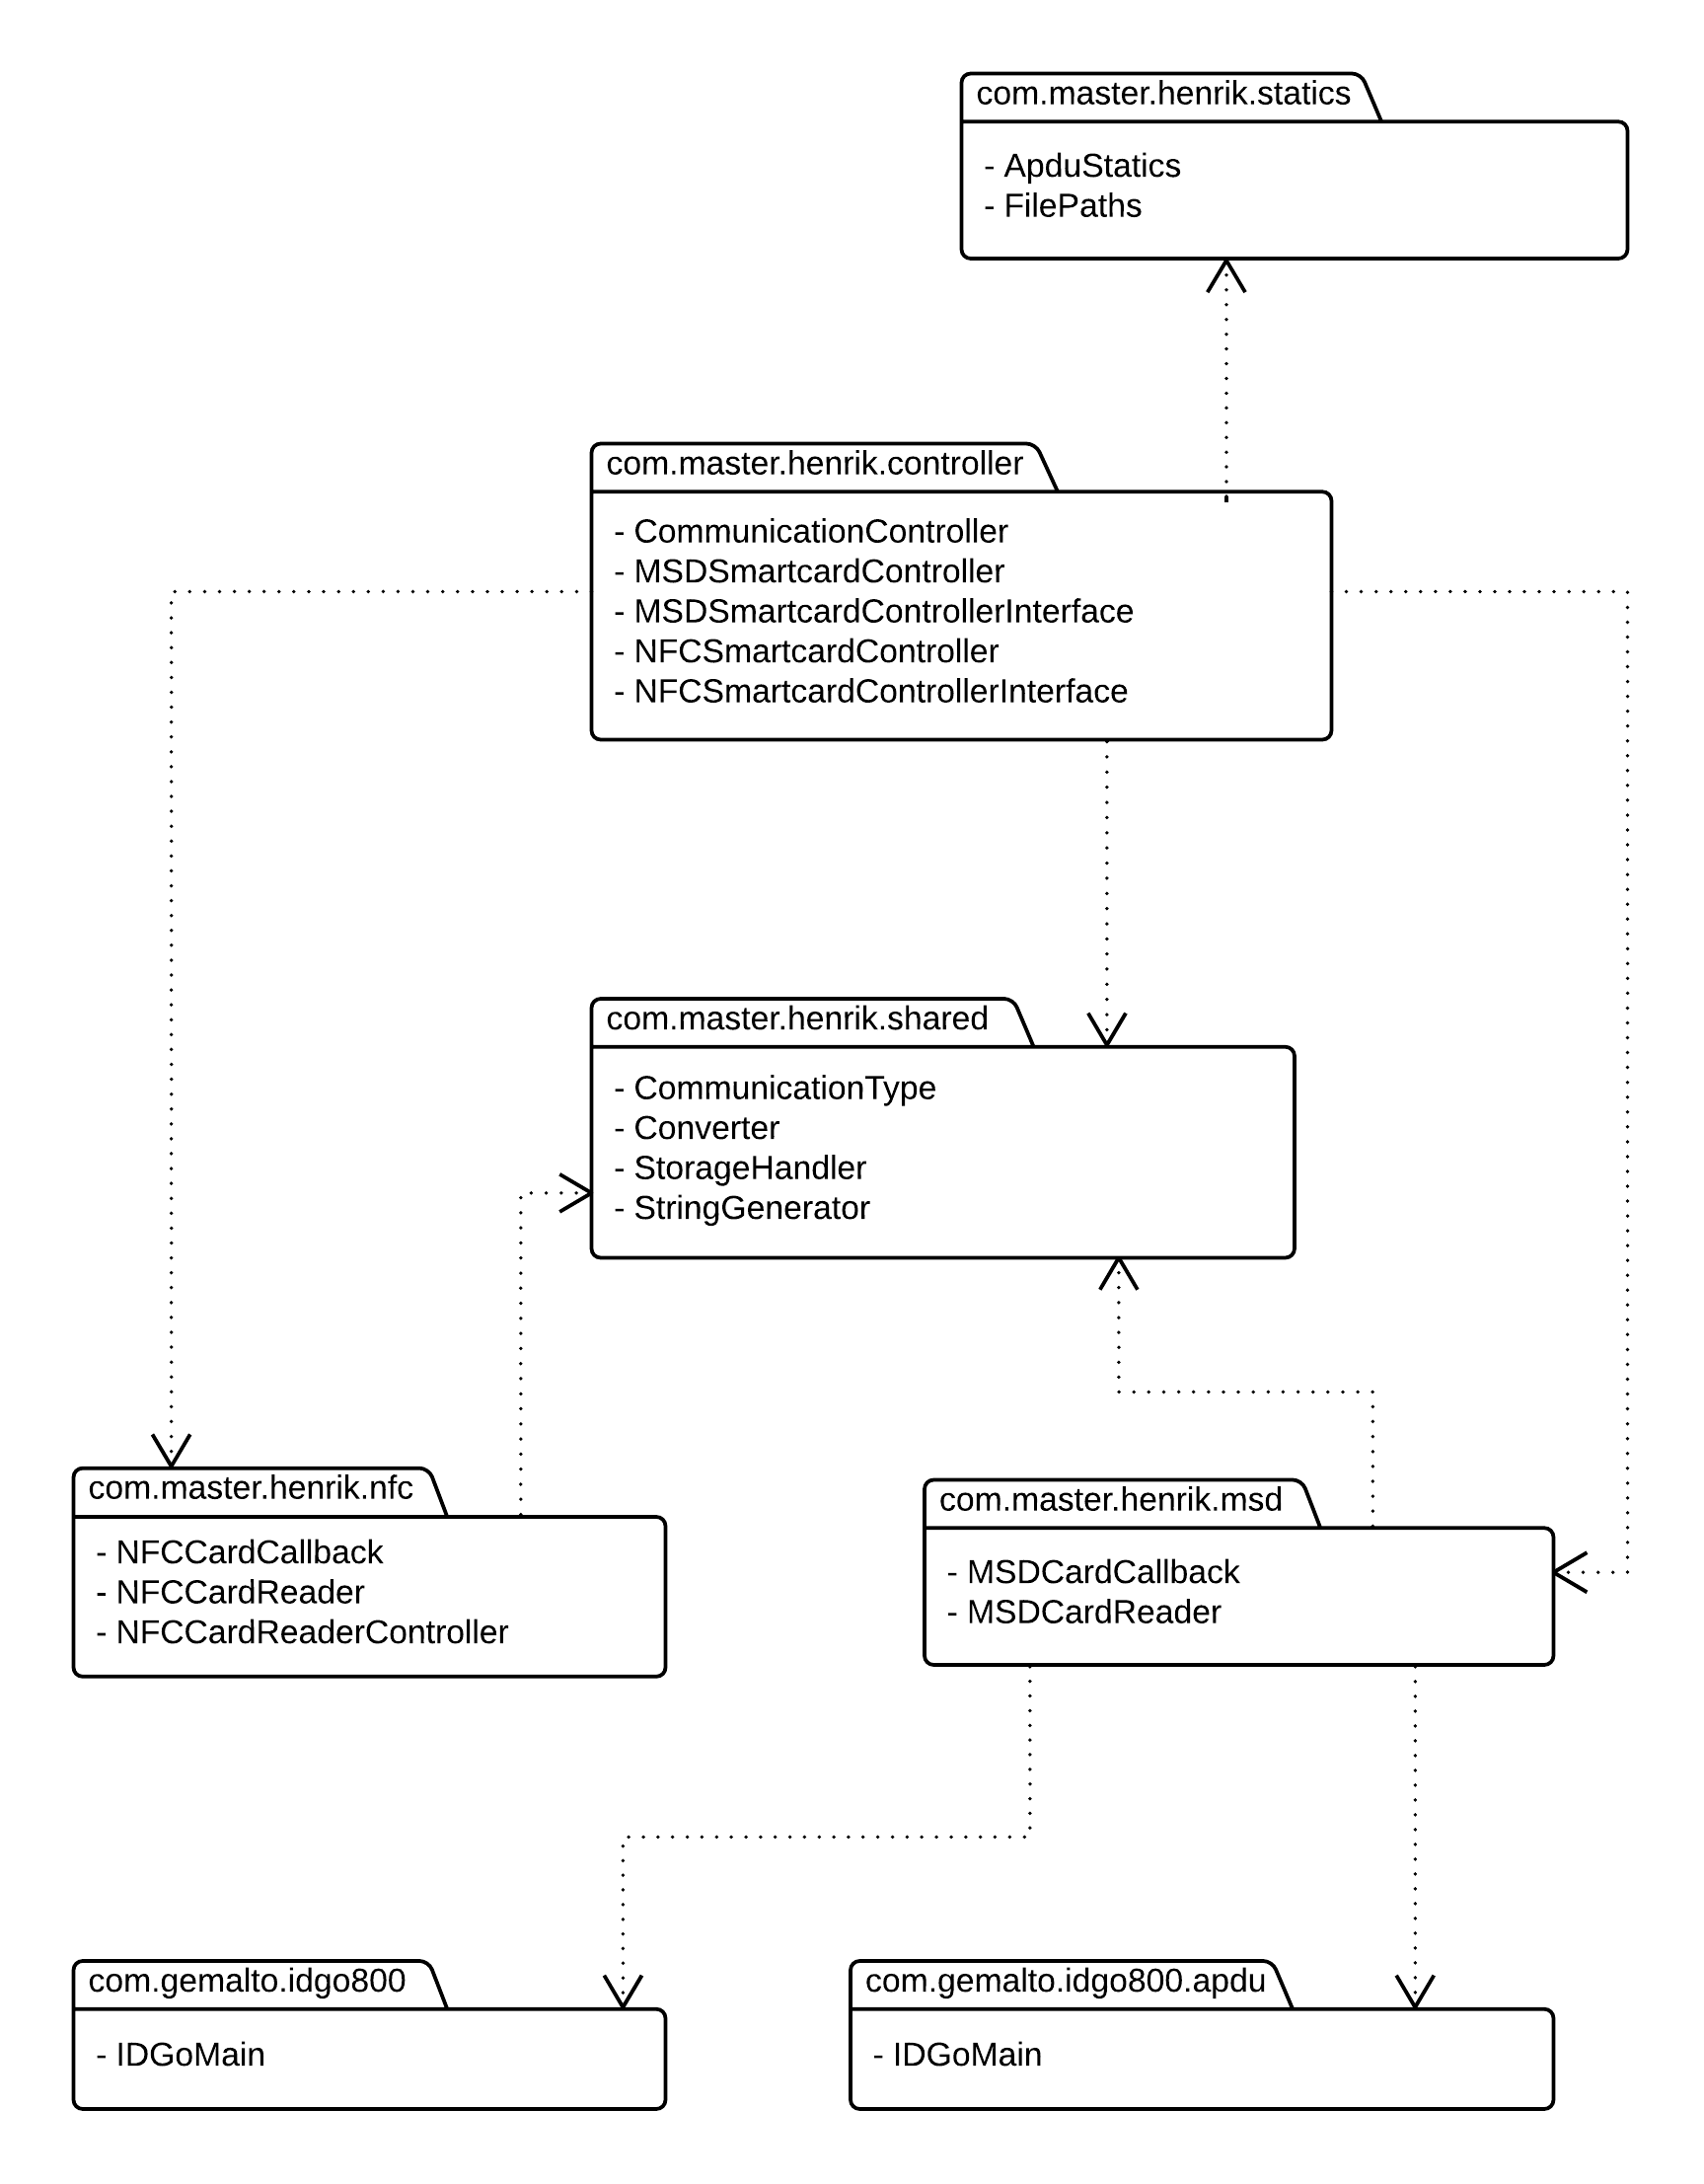
\includegraphics[width=0.95\textwidth]{images/package2.png}
\end{figure}

\subsection{Limitations}
\label{sec:limitationsMSD}
When we started testing the implementation it became evident that the micro SD smart card we had did not support extended APDU. As a result we are not able to perform tests that involve micro SD cards and extended APDU.
